%\begin{sidewaysfigure}
%  \begin{center}
%  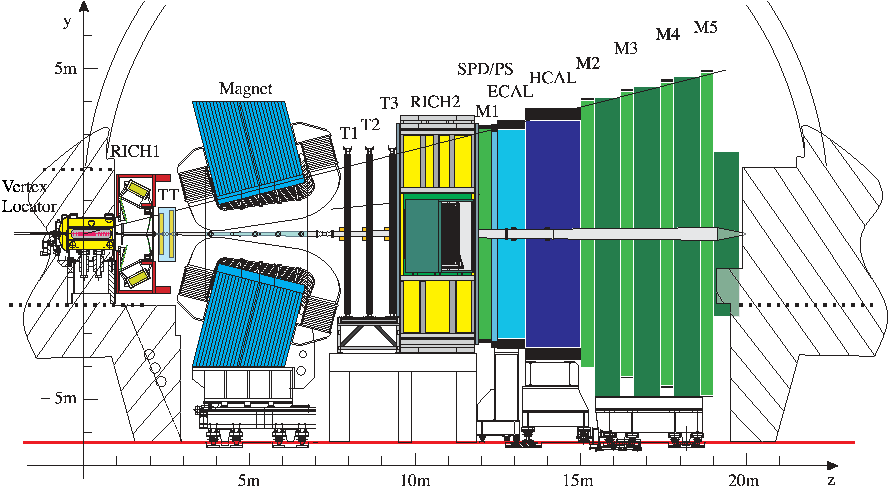
\includegraphics[width=0.8\textheight]{lhcb-detector-cross-section}
%  \caption[Cross-section view of \LHCb, cut in the non-bending $y$--$z$ plane]%
%    {Cross-section view of \LHCb, cut in the non-bending $y$--$z$ plane.}
%  \label{fig:LHCbCrossSection}
%  \end{center}
%\end{sidewaysfigure}



\chapter{ND280 ECal event reconstruction and software}
\label{chap:ND280Software}
The T2K experiment uses a bespoke software suite for simulation and analysis of ND280 data which is based on the ROOT framework~\cite{Brun199781}.  The vast majority of the ND280 software suite utilies these oaEvent library which provides a unified framework for information manipulation and was specifically designed for this purpose.
As ND280 consists of many subdetectors each providing a specific function, the ND280 software suite is designed to reflect this.  Not only are there specific software modules for individual subdetectors, there are specific modules for each phase of the subdetector information processing e.g. trip-T calibration, TPC reconstruction etc.  \newline
As the software suite handles both production of simulated data and the processing of collected data, there are sections of the processing chain which are specific to type of data being processed.  While the Monte Carlo simulation and real data do see different areas of the software chain, the general philosophy is to maniuplate the Monte Carlo or the real data to a point where they can be treated as equals and them process them in the same manner.  So, the description of the software will follow the same path: the Monte Carlo and real data specifics will be discussed first and then the unified treatment will follow. 
\section{Monte Carlo production software}
\label{sec:MCchain}
Process the MC

\subsection{Neutrino flux prediction}
\label{subsec:NeutrinoFluxPrediction}
I guess the flux is quite bit

\subsection{Neutrino interaction simulation}
\label{subsec:NeutrinoInteractionSimulation}
NEEEEEUT

\subsection{ND280 detector simulation}
\label{subsec:ND280DetectorSimulation}
nd280mc is really good for this

\subsection{Detector response simulation}
\label{subsec:DetectorResponseSimulation}
Is elecSim there?

\subsection{Detector calibration}
\label{subsec:DetectorCalibration}
oaCalib calibrates

\subsection{Event reconstruction}
\label{subsec:EventReconstruction}
oaRecon yo!


\section{Real data processing software}
\label{sec:datachain}
Process the data.  MAY NOT INCLUDE THIS


\section{ECal event reconstruction}
\label{sec:ECalEventReconstruction}
All about ecalRecon

\subsection{Hit preparation}
\label{subsec:ECalHitPerparation}
Hit prep

\subsection{Basic clustering}
\label{subsec:ECalBasicClustering}
Baaasic

\subsection{Cluster combination}
\label{subsec:ECalCombineClusters}
Combine dem clusters

\subsection{Cluster expansion}
\label{subsec:ECalExpandClusters}
Expand dem clusters

\subsection{3D cluster formation}
\label{subsec:ECal3DMatching}
Match the clusters

\subsection{3D hit reconstruction}
\label{subsec:ECal3DHitReconstruction}
Least square those fits

\subsection{Energy reconstruction}
\label{subsec:ECalEnergyReconstruction}
blah

\subsection{Event classification}
\label{subsec:ECalParticleIdentification}
Track or shower?
